\documentclass[11pt,a4paper]{article}
\usepackage[margin=2.1cm]{geometry}
\usepackage[T1]{fontenc}
\usepackage[utf8]{inputenc}
\usepackage{lmodern}
\usepackage{microtype}
\usepackage{graphicx}
\usepackage{booktabs}
\usepackage{array}
\usepackage{tabularx}
\newcolumntype{Y}{>{\raggedright\arraybackslash}X}
\usepackage{multirow}
\usepackage{amsmath}
\usepackage{xcolor}
\usepackage{enumitem}
\usepackage{tikz}
\usetikzlibrary{positioning,arrows.meta,shapes.misc}
\usepackage[font=small,labelfont=bf,skip=4pt]{caption}
\usepackage[backend=biber,style=numeric-comp,sorting=none,maxbibnames=3,minbibnames=3,giveninits=true,doi=true,url=false,isbn=false,eprint=false]{biblatex}
\addbibresource{references.bib}
\usepackage[colorlinks=true,linkcolor=blue!50!black,citecolor=blue!50!black,urlcolor=blue!50!black]{hyperref}
\usepackage{cleveref}
\setlist{nosep,leftmargin=1.4em}
\setlength{\parskip}{3pt}
\graphicspath{{figures/}}
\definecolor{box}{RGB}{235,242,250}
\newcommand{\vt}[1]{\texttt{#1}}

\title{\vspace{-1.2cm}\Large\textbf{Knowing when to look again:\\dynamic prediction of structural valve deterioration to personalise echocardiographic surveillance after bioprosthetic aortic valve replacement}}
\author{Team CardioNTUA\\\normalsize Athanasia Karagiannopoulou, Anna Panagiotakopoulou, Alexandros Barmperis (ML engineers) and Evangelie Sintou (clinician)\\\normalsize Dyania Health Hackathon 2026 \quad\textbullet\quad 17 September 2026}
\date{}

\begin{document}
\maketitle
\vspace{-0.9cm}
\begin{abstract}
\noindent Bioprosthetic aortic valves deteriorate, and every patient is followed with the same annual echocardiogram whatever their risk. Two facts make this wasteful and unsafe: a single-echo diagnosis of structural valve deterioration (SVD) disappears at the next visit in 59--65\% of patients, and late recognition turns elective reintervention into an urgent one. We propose a study protocol for \emph{dynamic} prediction of confirmed VARC-3 moderate SVD at every follow-up echo, with death as a competing risk, and turn the prediction into a risk-adapted echo schedule. Because no public dataset holds serial prosthetic-valve echoes with valve model, we built a prototype on a synthetic cohort of 10,000 valves: individual-patient curves reconstructed from three published cohorts, valve physics anchored to the 2024 ASE normal-value tables, and echo noise calibrated to the published label-flicker statistics. On held-out synthetic valves the dynamic model reached a 5-year AUC of 0.875 (95\% CI 0.851--0.899) on echoes not already abnormal, against 0.651 for time since implant; a 1\% risk rule used 44\% fewer echoes than guideline surveillance with a confirmation echo, at +0.7 months mean detection delay. Against the noise-free truth the confirmed VARC-3 label detects only 60\% of true deteriorations with a 1.5-year median lag, an audit no registry can perform. A face-validity check on the provided de-identified notes reproduced the label rule's behaviour but cannot validate the models; that requires the data the protocol requests.
\end{abstract}

\section{The clinical problem}

\paragraph{Bioprosthetic valves wear out.} Surgical (SAVR) and transcatheter (TAVR) bioprostheses are now implanted in younger patients with longer life expectancy, so durability has become the central question of aortic valve therapy \cite{trimaille2025}. Leaflets stiffen and calcify through lipid infiltration, immune response to xenogeneic tissue, mechanical fatigue and thrombosis; a minority fail by cusp tear and regurgitation \cite{kostyunin2020,wakami2022}. The end point is bioprosthetic valve failure (BVF) and reintervention, by redo surgery or valve-in-valve TAVR, with different patients routed to each \cite{geisler2026}; annual valve-in-valve volume in the United States is projected to reach roughly 42,000 procedures by 2035 \cite{genereux2025}.

\paragraph{How SVD is defined.} Three consensus definitions stage haemodynamic SVD from echocardiography: EAPCI/ESC/EACTS 2017 \cite{capodanno2017}, Dvir 2018 \cite{dvir2018} and VARC-3 \cite{genereux2021}. VARC-3 moderate (stage~2) SVD is a mean gradient $\geq 20$ mmHg \emph{and} a rise $\geq 10$ mmHg from the early post-implant echo, with a fall in effective orifice area (EOA) or dimensionless velocity index (DVI), or new moderate intraprosthetic regurgitation (criteria adopted unchanged by the 2025 ESC/EACTS guideline \cite{praz2025}); severe (stage~3) is $\geq 30$ mmHg with a rise $\geq 20$ mmHg, or severe regurgitation. All three define SVD as a \emph{change} from a reference echo, not an absolute threshold. Thresholds for prosthesis--patient mismatch (PPM) and the normal EOA, gradient and DVI of each valve model and size are tabulated in the 2024 ASE prosthetic-valve guideline \cite{zoghbi2024}.

\paragraph{What is known about the rates.} In the NOTION trial at ten years, moderate-or-worse SVD occurred in 15.4\% of TAVI and 20.8\% of SAVR patients, severe SVD in 1.5\% vs 10.0\% \cite{thyregod2024}. In 338 Magna Ease valves followed with annual echo, freedom from VARC-3 stage 2/3 SVD was 98.5\% at five years and 60.9\% at ten \cite{kermen2022}. Across 12,569 Perimount implants, explant for SVD depended steeply on age at implant \cite{johnston2015}; in 1,387 surgical valves, 31\% showed haemodynamic deterioration, mostly subclinical \cite{salaun2018}. PPM, small orifice, younger age, smoking, diabetes and renal failure raise the hazard \cite{trimaille2025,wakami2022}. Subclinical degeneration is detectable years before the echo changes \cite{cartlidge2019}.

\paragraph{Problem 1: the label is noisy.} In 1,118 patients with one valve model and core-laboratory echoes, the three definitions flagged 4.6\%, 2.9\% and 3.0\% of patients by five years, and \textbf{59--65\% of first SVD classifications had vanished at the next visit} \cite{velders2024}. Doppler gradients depend on flow, alignment and outflow-tract measurement, so a single threshold crossing is as often noise as disease. Any prediction model trained on single-echo labels learns the noise.

\paragraph{Problem 2: surveillance is one-size-fits-all.} Guidelines ask for an echo within three months of implantation, at one year and annually thereafter for everyone \cite{praz2025}; the 2021 edition set the baseline within 30 days \cite{vahanian2021}, and the American guideline is similar \cite{otto2021}. Low-risk valves receive echoes they do not need; rising trajectories wait for the next annual slot; and an abnormal echo has no formal confirmation rule. Late recognition matters: emergency redo surgery carries 22.6\% mortality against 1.4\% for elective redo \cite{cartlidge2019}. Adjacent fields have already moved to risk-stratified imaging surveillance \cite{hofmann2024}, and joint longitudinal--survival models give a principled way to choose the next measurement time \cite{rizopoulos2016}.

\paragraph{Our proposal.} A study protocol whose model, updated at every echo, predicts the cumulative incidence of \emph{confirmed} moderate SVD over the next 0.5--5 years with death as a competing risk, and whose output is the next echo interval. The prototype shows that the design works, where it breaks, and how much the label itself costs.

\section{Study design in brief}

\textbf{Objectives.} Primary: predict an individual's time to confirmed moderate-or-greater haemodynamic SVD accurately enough to personalise the surveillance interval. Secondary: (1) SAVR vs TAVR and valve-model trajectories; (2) a risk-adapted schedule vs the guideline schedule on echoes used and detection delay; (3) the reintervention window from first confirmed moderate SVD to severe SVD or reintervention, and the urgent share; (4) agreement and persistence of the VARC-3, Capodanno and Dvir labels.

\textbf{Population.} Adults with a first bioprosthetic SAVR or TAVR, valve model and size recorded, a reference echo within three months (or a model~$\times$~size reference value, flagged) and at least one follow-up echo. Excluded: mechanical valves, homografts, Ross, index valve-in-valve, concomitant mitral or tricuspid prostheses, active endocarditis at implant. Endocarditis, thrombosis and paravalvular leak \emph{during} follow-up are competing events or covariates, not exclusions.

\textbf{Primary endpoint.} Time from the reference echo to VARC-3 stage $\geq 2$ SVD \textbf{confirmed on two consecutive echoes}, competing with death, endocarditis and non-SVD reintervention; SVD reintervention before the confirming echo counts as an event. Ground-truth hierarchy: explant pathology $>$ reintervention with SVD indication $>$ confirmed VARC-3 echo criteria $>$ blinded heart-team adjudication. \textbf{Secondary endpoints:} BVF, reintervention (elective vs urgent), annualised gradient progression, surveillance performance.

\textbf{Data sources for deployment.} Echo reporting database (serial measurements), STS Adult Cardiac Surgery Database and STS/ACC TVT Registry (device, comorbidities, 30-day echo), EHR with transformer-based extraction of notes \cite{xie2026}, CMS/NDI linkage for out-of-system reintervention and death. Target $\geq 5{,}000$ development and $\geq 2{,}000$ external-validation valves, chosen from the events-per-parameter rule \cite{riley2020} and a simulation-based precision curve (\cref{sec:results}).

\textbf{Usefulness thresholds, fixed in advance.} Statistical: time-dependent AUC $\geq 0.75$, C-index $\geq 0.70$ at five years, calibration slope 0.8--1.2. Decision level: $\geq 25\%$ fewer echoes per patient-decade with mean and 90th-percentile detection delay no more than three months longer than guideline surveillance. Reporting follows TRIPOD+AI \cite{collins2024}; competing risks are reported as recommended by Austin and Fine \cite{austin2017}.

\section{Why we simulate, and how}\label{sec:sim}

No public dataset contains serial prosthetic-valve echoes with valve model and adjudicated events, and the de-identified extracts provided for the hackathon (117 patients, year-only dates, redacted ages, one note per follow-up) cannot support a time-to-event model (\cref{sec:real}). We therefore built a simulator whose every parameter is either sourced or flagged as an assumption, calibrated it to published curves, and used it for three things a real registry cannot do: test the design end to end, compare each label definition with the noise-free truth, and run surveillance policies on identical patients. \Cref{fig:pipeline} shows the pipeline.

\begin{figure}[t]
\centering
\resizebox{\textwidth}{!}{%
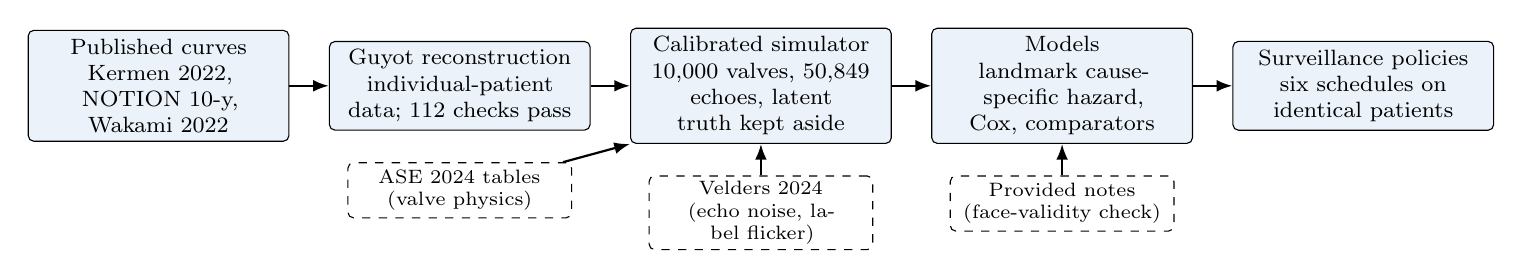
\begin{tikzpicture}[node distance=4mm and 5mm, every node/.style={font=\footnotesize},
  b/.style={draw, rounded corners=2pt, fill=box, align=center, minimum height=9mm, text width=31mm, inner sep=3pt},
  s/.style={draw, dashed, rounded corners=2pt, align=center, minimum height=7mm, text width=27mm, inner sep=2pt, font=\scriptsize},
  a/.style={-{Latex[length=2mm]}, thick}]
\node[b] (pub) {Published curves\\Kermen 2022, NOTION 10-y, Wakami 2022};
\node[b, right=of pub] (rec) {Guyot reconstruction\\individual-patient data; 112 checks pass};
\node[b, right=of rec] (sim) {Calibrated simulator\\10,000 valves, 50,849 echoes, latent truth kept aside};
\node[b, right=of sim] (mod) {Models\\landmark cause-specific hazard, Cox, comparators};
\node[b, right=of mod] (pol) {Surveillance policies\\six schedules on identical patients};
\node[s, below=of rec] (ase) {ASE 2024 tables\\(valve physics)};
\node[s, below=of sim] (vel) {Velders 2024\\(echo noise, label flicker)};
\node[s, below=of mod] (notes) {Provided notes\\(face-validity check)};
\draw[a] (pub) -- (rec); \draw[a] (rec) -- (sim); \draw[a] (sim) -- (mod); \draw[a] (mod) -- (pol);
\draw[a] (ase) -- (sim.south west); \draw[a] (vel) -- (sim); \draw[a] (notes) -- (mod);
\end{tikzpicture}}
\caption{From published evidence to a testable prototype. Solid boxes are the pipeline; dashed boxes are external anchors.}
\label{fig:pipeline}
\end{figure}

\subsection{Reconstructing individual-patient data from published curves}
Durability papers publish Kaplan--Meier or cumulative-incidence curves with numbers at risk. The Guyot algorithm \cite{guyot2012} inverts these into a patient-level time-to-event dataset that reproduces the curve and the risk table. We automated it for three sources: Kermen 2022 (Magna Ease, $n=338$; vector PDF, so curves, censor marks and risk rows were parsed from the drawing commands with no manual input) \cite{kermen2022}, the NOTION 10-year figure (TAVI $n=134$, SAVR $n=123$; raster image, risk rows typed from the figure) \cite{thyregod2024} and Wakami 2022 (Trifecta, $n=110$) \cite{wakami2022}. Every published anchor is a test: 112 checks pass, and the primary-label curve reproduces its risk row (338/247/34/20) and its 49 events exactly (\cref{fig:guyot}).

\begin{figure}[t]
\centering
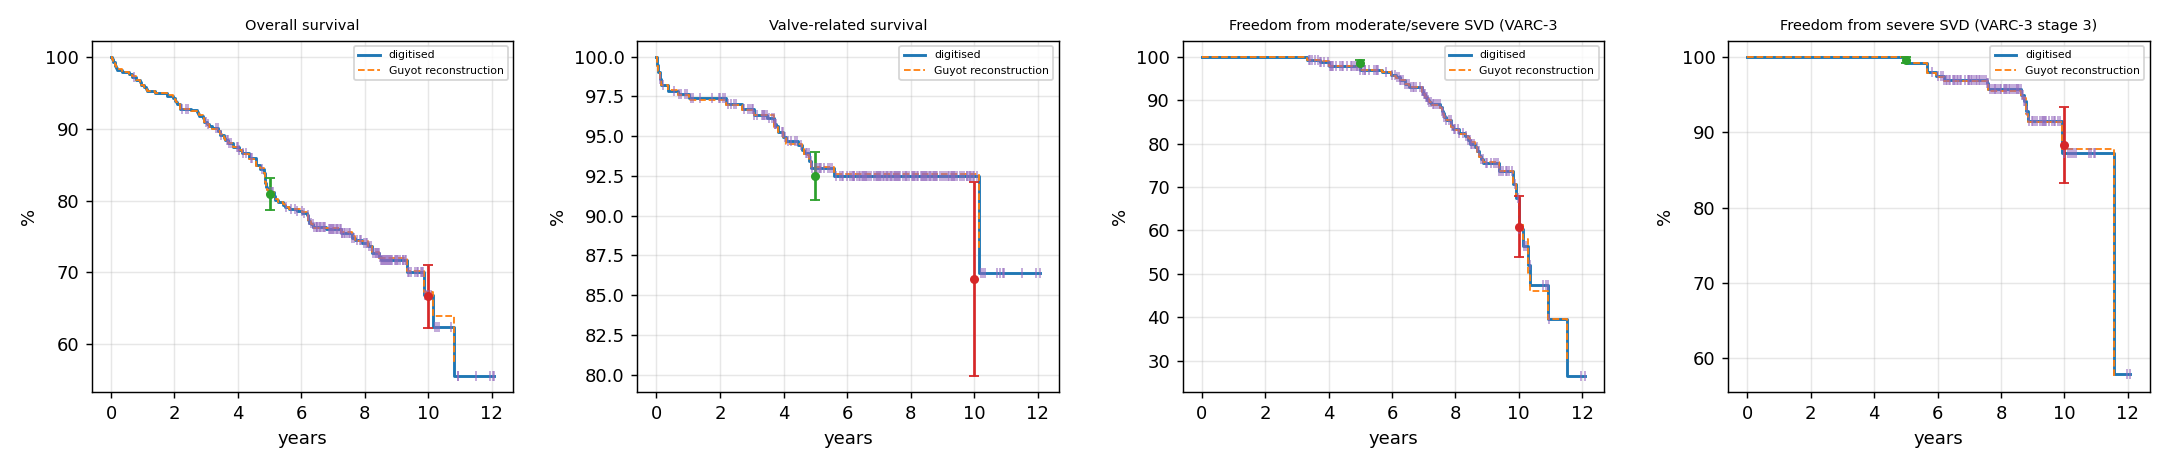
\includegraphics[width=\textwidth]{qa_kermen_fig2}
\caption{Kermen 2022, Figure 2, reconstructed. Blue: the digitised published curve with censor marks; orange: the Guyot reconstruction; dots with bars: the published 5- and 10-year values with their confidence intervals.}
\label{fig:guyot}
\end{figure}

\subsection{The generative model}
The object simulated is one valve from implant to reintervention, death or censoring, with a hidden state observed through noisy, irregularly timed echoes.

\begin{itemize}
\item \textbf{One latent state.} The true effective orifice area $\mathrm{EOA}^*(t)$ is the only quantity that degenerates. Mean gradient, peak velocity and DVI follow from flow physics, $\mathrm{MPG} = c\,(Q/\mathrm{EOA}_{\mathrm{eff}})^2$ with $\mathrm{EOA}_{\mathrm{eff}} = \mathrm{EOA}\,(Q/Q_{\mathrm{ref}})^{0.35}$ and $\mathrm{DVI} = \mathrm{EOA}/A_{\mathrm{LVOT}}$, with $c$ fitted per valve model and size to the ASE 2024 normal-value tables \cite{zoghbi2024}. Label flicker, regression to the mean and disagreement between definitions therefore \emph{emerge} from measurement error; nothing is injected.
\item \textbf{Onset and progression.} Deterioration starts at $T_{\mathrm{deg}}$, drawn from a proportional-hazards Weibull per valve class (Perimount-class, Trifecta-class, porcine/Mitroflow, balloon-expandable, self-expanding, and a ``new valve'' class with little history). Only biological effects enter the hazard (smoking 2.58, diabetes 1.33, BMI 1.08 per unit, CKD 1.3, age 0.951 per year for surgical valves, anticoagulation and thrombosis effects). Effects with a mechanical pathway (PPM, small transcatheter valve, high baseline gradient) act through the reference orifice area and are checked afterwards as \emph{emergent} hazard ratios, so nothing is counted twice. After onset the orifice shrinks exponentially with a valve-specific time constant; 25\% of surgical and 60\% of Trifecta degenerations take a regurgitant path (cusp tear). Transient leaflet thrombosis in the first year (8\% TAVR, 3\% SAVR, halved on anticoagulation) reduces the orifice for 3--9 months and then resolves: it is not SVD, and it tests the specificity of each label.
\item \textbf{The echo.} Four independent per-visit error sources with the correct cross-channel structure: flow state (gradient $\propto f^2$, EOA and DVI unchanged), LVOT velocity sampling, continuous-wave alignment, and LVOT diameter (enters EOA squared), plus a persistent per-valve LVOT bias that cancels in changes from reference. Regurgitation grades are misclassified by one grade with probability 0.03; EOA is missing in 8\% and DVI in 5\% of echoes.
\item \textbf{Visits and competing events.} Reference echo at 30 days (inside the guideline's three-month window), then one year and annually \cite{praz2025}, with missingness rising from 9\% at year one to 35\% at year four \cite{velders2024}, higher when the patient feels well and lower when symptomatic; symptom-triggered echoes; death by an attained-age Gompertz hazard with frailty; endocarditis; reintervention only after \emph{detected} severe SVD or symptomatic moderate SVD, less likely with age, urgent if first detected at a symptom-triggered echo. Because reintervention depends on detection, a surveillance policy has consequences.
\item \textbf{Labels.} Capodanno, Dvir and VARC-3 (full and the haemodynamic variant used by NOTION), each as single-echo and confirmed (same or higher stage at the next echo). An \emph{oracle} label applies the same rules to the noise-free channels, and the continuous-time crossing of the true stage-2 threshold is stored for the delay metric. The latent truth is never used for training.
\end{itemize}

\subsection{Calibration: fit to what the papers measured}
The reconstructed curves are \emph{observed}, visit-timed labels, not the latent onset distribution. Calibration therefore simulates a cohort matched to each paper's baseline table (age, sizes, PPM, valve class, reference-echo timing, schedule, completeness, mortality), applies the paper's own single-echo label rule and estimator (Kaplan--Meier with death censored for Kermen, Aalen--Johansen elsewhere), and adjusts the latent Weibull until the simulated observed curve matches. The order is sequential and over-identified: physics constants $\to$ echo noise on a PERIGON-like cohort against Velders' regression-to-the-mean deciles \cite{velders2024} $\to$ mortality on Kermen's survival curve $\to$ onset per class. Kermen fixes the Perimount class, Wakami the Trifecta class and NOTION TAVI the self-expanding class; the NOTION surgical arm at age 79 is then \emph{predicted with no free parameter} by transporting the surgical classes through the age hazard, before the porcine share is freed. \Cref{tab:calib} and \cref{fig:calib} give the result; the confirmed two-echo primary endpoint is an output, never a target.

\begin{table}[t]
\centering\small
\caption{Calibration and validation targets (percent). Fits are the maximum absolute deviation over the years with at least 30 at risk.}
\label{tab:calib}
\footnotesize
\begin{tabularx}{\textwidth}{@{}Ylll@{}}
\toprule
Target & Published & Simulated & Verdict \\
\midrule
Kermen freedom from VARC-3 stage 2/3 at 5 / 10 y (KM) \cite{kermen2022} & 97.0 / 63.8 & 96.9 / 62.9; max 1.4 pp & pass \\
Wakami Trifecta SVD at 5 / 7 y (AJ) \cite{wakami2022} & 4.8 / 6.3 & max 2.0 pp & pass \\
NOTION TAVI $\geq$moderate SVD at 10 y (AJ) \cite{thyregod2024} & 15.4 & 13.2; max 2.8 pp & pass \\
NOTION SAVR $\geq$moderate SVD at 10 y, \textbf{predicted with no free parameter} & 20.7 & 21.6; max 3.1 pp & pass \\
Kermen freedom from stage 3 at 10 y (progression speed) & 87.2 & 85.3 & pass \\
Kermen explant for SVD at 10 y & 8.4 & 8.1 & pass \\
NOTION severe SVD at 10 y, SAVR / TAVI & 9.9 / 1.4 & 14.1 / 5.1 & miss (3.7--4.1 pp) \\
Kermen overall survival, 1--10 y & curve & max 2.0 pp & pass \\
Velders ever-labelled by 5 y, Capodanno / Dvir / VARC-3 \cite{velders2024} & 4.6 / 2.9 / 3.0 & 4.3 / 2.9 / 4.0 & pass \\
Velders VARC-3 persistence at the next visit & 35--41 (range 14--50) & 20 & pass \\
Velders 95\% interval of 5-y within-patient gradient change & $(-9.6, +7.5)$ & $(-9.1, +9.3)$ & pass \\
\bottomrule
\end{tabularx}
\end{table}

\begin{figure}[t]
\centering
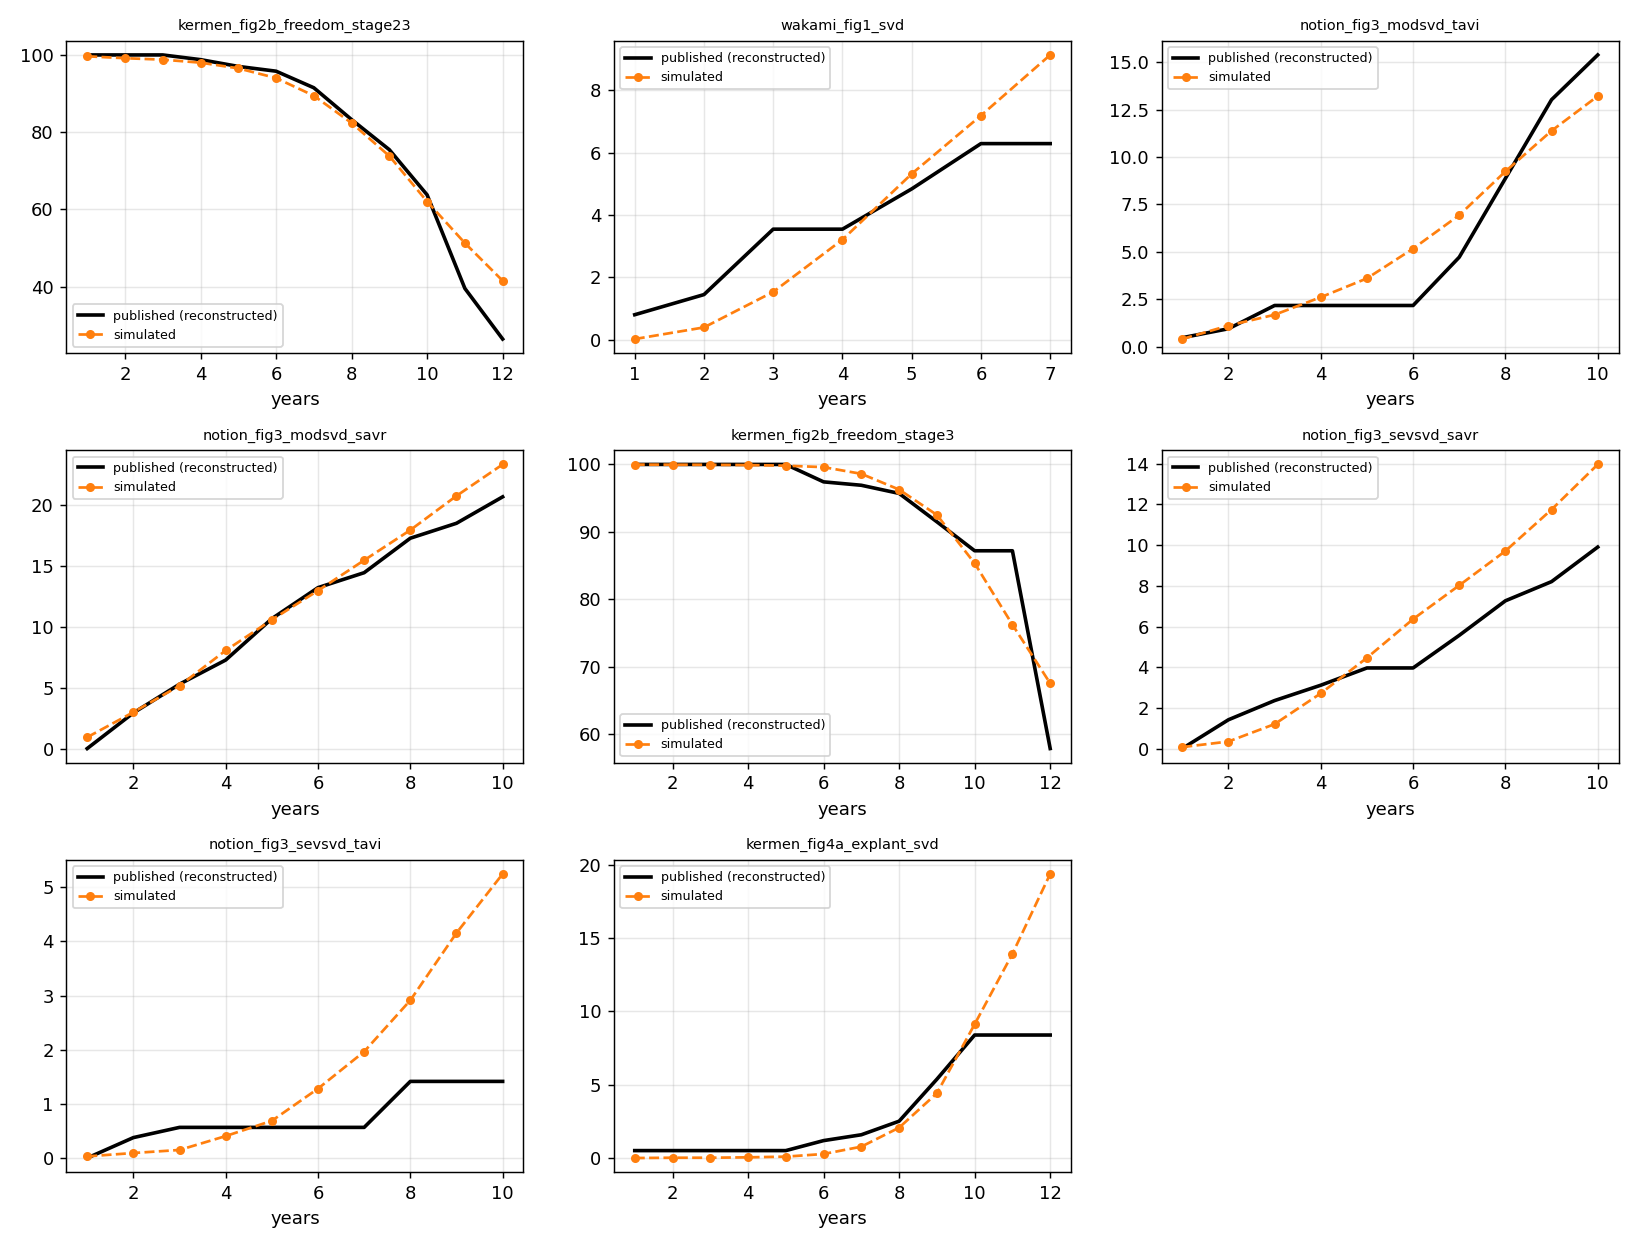
\includegraphics[width=0.9\textwidth]{curves_sim_vs_target}
\caption{Simulated observed-label curves (orange) against the reconstructed published curves (black). The three targets fitted are Kermen stage 2/3, Wakami and NOTION TAVI; NOTION SAVR moderate SVD was predicted before its porcine share was freed; the stage-3, severe-SVD and explant panels are checks on progression speed. Severe SVD runs too fast at ten years (the two documented misses).}
\label{fig:calib}
\end{figure}

\textbf{What we accept as imperfect.} Of 40 calibration checks two fail and of 37 acceptance checks seven miss, all documented: severe SVD progresses 3.7--4.1 points too fast at ten years; three emergent hazard ratios (baseline gradient, small transcatheter valve, smoking) are weaker than published, which is expected because published hazard ratios were estimated on noisy labels; simulated PPM prevalence is 40\% vs 51\%; per-model gradients deviate from the ASE rows by at most 3.8 mmHg. Assumptions that favour the model are stated: symptoms occur only with true deterioration, death is independent of SVD, and there are no site or vendor effects.

\textbf{The cohort.} 10,000 valves (5,441 SAVR, 4,559 TAVR), 50,849 echoes, 1,641 confirmed VARC-3 stage-$\geq 2$ events, 4,009 deaths, 1,589 reinterventions and 572 endocarditis episodes; confirmed cumulative incidence 6.2\%, 11.3\% and 16.8\% at 5, 8 and 10 years. Every column maps to an STS, TVT or echo-database field, so the analysis code runs unchanged on real data. \Cref{fig:flicker} shows why the label needs care.

\begin{figure}[t]
\centering
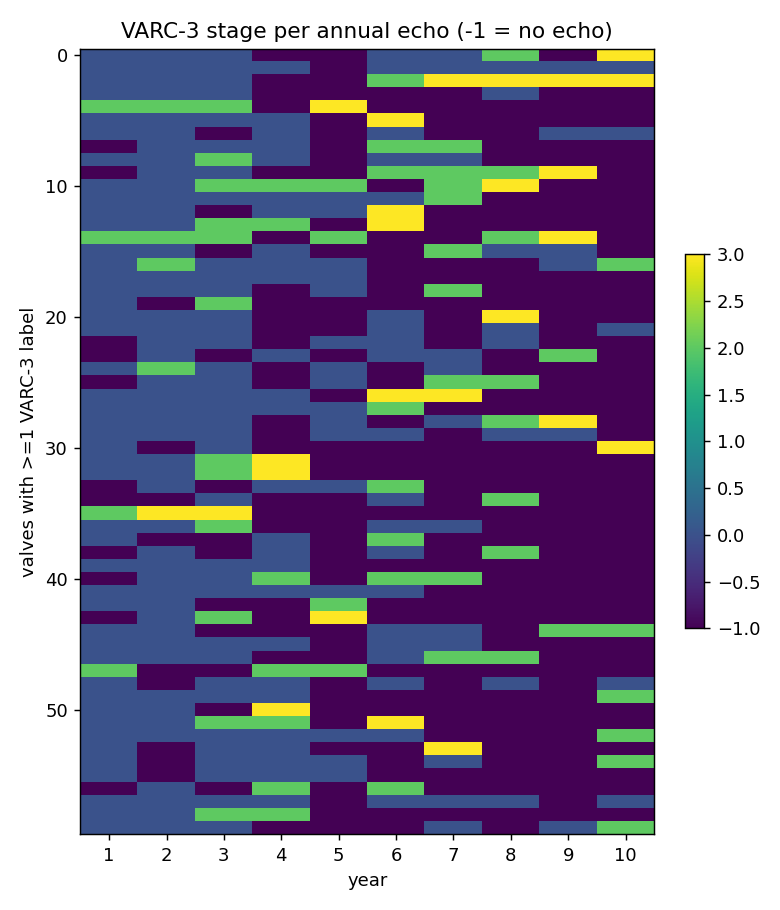
\includegraphics[width=0.46\textwidth]{label_flicker_heatmap}
\caption{Sixty simulated valves with at least one VARC-3 label: stage per annual echo (blue 0, green 2, yellow 3, dark purple no echo). Isolated stage-2 echoes that revert are the flicker Velders et al.\ measured \cite{velders2024}; the confirmed label requires two consecutive abnormal echoes.}
\label{fig:flicker}
\end{figure}

\section{The prediction model}\label{sec:model}

\paragraph{Landmark design.} Every post-reference echo is a decision point. From everything known at that echo (baseline, reference and the echo history so far) the model predicts the cumulative incidence of confirmed moderate SVD over the next 0.5--5 years, with death, endocarditis and non-SVD reintervention as competing causes. A confirmed label exists only at the second abnormal echo, a median 0.94 years after the first, so the outcome is dated at the \emph{confirming} echo: a prediction never uses information from its own future. Instances from one valve overlap, so every split, early-stopping fold and bootstrap is by valve (70/15/15). An implant-time version predicts 5/8/10-year incidence from the reference echo for protocol reporting.

\paragraph{Discrete-time cause-specific hazard.} Follow-up after each landmark is cut into 6-month periods $j$, and a gradient-boosted multinomial classifier (scikit-learn \vt{HistGradientBoostingClassifier}) estimates per period the cause-specific hazards $h_{1j}$ (SVD) and $h_{2j}$ (competing) from the features, the period index and the landmark time. Event-free survival is $S_j = \prod_{l\le j}(1-h_{1l}-h_{2l})$ and the cumulative incidence over $\Delta$ years is $\mathrm{CIF}_1(\Delta) = \sum_{j \le \Delta/0.5} S_{j-1}\,h_{1j}$. This handles censoring by construction, gives calibrated probabilities without resampling, allows nonlinear trajectory effects, handles missing values natively, trains in seconds and scales linearly to registry volumes. The same quantity answers the surveillance question directly: what is the risk before the next echo if we wait 6, 12, 24 or 36 months? Cause-specific Cox models with Aalen--Johansen incidence supply hazard ratios for clinical review; deep survival models \cite{lee2018,wiegrebe2023}, random survival forests \cite{ishwaran2008} and joint models \cite{rizopoulos2016} are the next step at registry scale, and periodic recalibration is planned because static risk models in this population drift \cite{pollack2023}.

\paragraph{Features.} A variable enters only with a quantified effect or a defined role and a field on the STS/TVT forms. Baseline: age, sex, BSA, BMI, diabetes, CKD/dialysis, smoking, atrial fibrillation, anticoagulant type, approach, valve model and class, size, implant year, reference gradient, EOA, indexed EOA, DVI, PPM class, and whether the reference came from an echo or the model~$\times$~size table. Engineered from the echo history: change in gradient from reference (the VARC-3 quantity), current single-echo VARC-3 stage and count of prior abnormal echoes (the ``unconfirmed abnormal echo'' flag), an exponentially weighted mean of the log gradient with the posterior probability that the true gradient exceeds 20 mmHg (Doppler error is multiplicative), slope since reference and over the last two echoes, running maximum, consecutive-worsening count and transient-spike flag, relative EOA and DVI change, expected EOA for the model and size with its residual \cite{zoghbi2024}, time since last echo, number of echoes and a symptom-triggered flag. A registry-only subset isolates the value of the engineered features.

\paragraph{Comparators and metrics.} Time since implant alone (what guideline surveillance implicitly assumes); a Cox model with the published risk-factor set (age, sex, BMI, diabetes, smoking, CKD, PPM, baseline gradient, size, anticoagulation \cite{trimaille2025}); the registry-only feature set. Cause-specific time-dependent AUC at 3 and 5 years from each echo and 5/8/10 years from implant, the truncated cause-specific C-index \cite{uno2011}, Brier score and decile calibration with a logistic recalibration slope, all with 500 valve-level bootstrap resamples paired across models. Metrics are also reported on echoes that are not already abnormal, because that is where a scheduling decision is made. SHAP values give global importance and the per-patient top-3 drivers; backward elimination along permutation importance gives a parsimonious deployment model.

\section{The surveillance experiment}\label{sec:policy}

Six schedules were run on the \emph{same} simulated patients with common random numbers: the $k$-th echo of a valve sees the same measurement noise under every policy, and reintervention luck is pre-drawn, so differences between policies are differences in the schedule alone. All policies include a confirmation echo 3--6 months after any single abnormal echo, so the model's contribution is separated from the confirmation rule's. Policies: guideline (30 days, 1 year, annual); guideline plus confirmation; rule-based de-escalation after stable echoes; time-since-implant only; \textbf{risk-adapted}, which chooses the longest interval among 6, 12, 18, 24 and 36 months whose predicted confirmed-SVD risk stays below a threshold $\tau$ (severe-SVD risk below $2\tau$), swept over $\tau$; and an oracle that sees the latent truth, marking the best any schedule could do. Symptoms always trigger an echo. Metrics: echoes per patient-decade, delay from the true stage-2 crossing to confirmed detection (mean and 90th percentile), share of true deteriorations detected, share of severe SVD first seen while still moderate, and urgent reinterventions.

\section{Results on the synthetic cohort}\label{sec:results}

\subsection{Prediction}
On the 1,401 test valves (6,251 landmark instances) the dynamic model passed every pre-specified threshold (\cref{tab:models}, \cref{fig:auc}). Its 5-year AUC was 0.925 on all echoes and 0.875 on echoes not already abnormal; time since implant alone gave 0.651 there. Calibration was close to the diagonal across deciles (\cref{fig:calib5}). The registry-only feature set lost only 0.003 AUC: the gain comes from the dynamic framing and the label handling, not from feature engineering. Eight features (valve model, time since implant, approach, current stage, change in gradient, age, haemodynamic stage, smoking) reached 0.924. At implant time the boosted model beat the published risk-factor Cox at every horizon (0.865/0.850/0.823 vs 0.756/0.756/0.771 at 5/8/10 years).

\begin{table}[t]
\centering\small
\caption{Test-set discrimination and calibration (valve-level bootstrap, 500 resamples).}
\label{tab:models}
\footnotesize
\begin{tabularx}{\textwidth}{@{}Yrccc@{}}
\toprule
Model & Instances & AUC at 5 y (95\% CI) & C at 5 y & Calib.\ slope \\
\midrule
Dynamic model, all echoes & 6,251 & 0.925 (0.911--0.939) & 0.919 & 0.96 \\
Dynamic model, echoes not already abnormal & 5,555 & \textbf{0.875 (0.851--0.899)} & 0.855 & 1.04 \\
\quad registry-only features & 5,555 & 0.872 (0.848--0.896) & 0.854 & 1.05 \\
\quad time since implant only & 5,555 & 0.651 (0.614--0.686) & 0.638 & 0.87 \\
Implant-time boosted model, 5 / 8 / 10 y & 1,489 & 0.865 / 0.850 / 0.823 & 0.844 / 0.817 / 0.783 & 0.94 / 0.95 / 0.96 \\
Cause-specific Cox, full baseline, 5 / 8 / 10 y & 1,489 & 0.814 / 0.809 / 0.810 & 0.784 / 0.762 / 0.750 & 1.21 / 1.17 / 1.08 \\
Published risk-factor Cox, 5 / 8 / 10 y & 1,489 & 0.756 / 0.756 / 0.771 & 0.723 / 0.705 / 0.699 & 1.05 / 0.99 / 0.98 \\
\bottomrule
\end{tabularx}
\end{table}

\begin{figure}[t]
\centering
\begin{minipage}[t]{0.58\textwidth}\centering
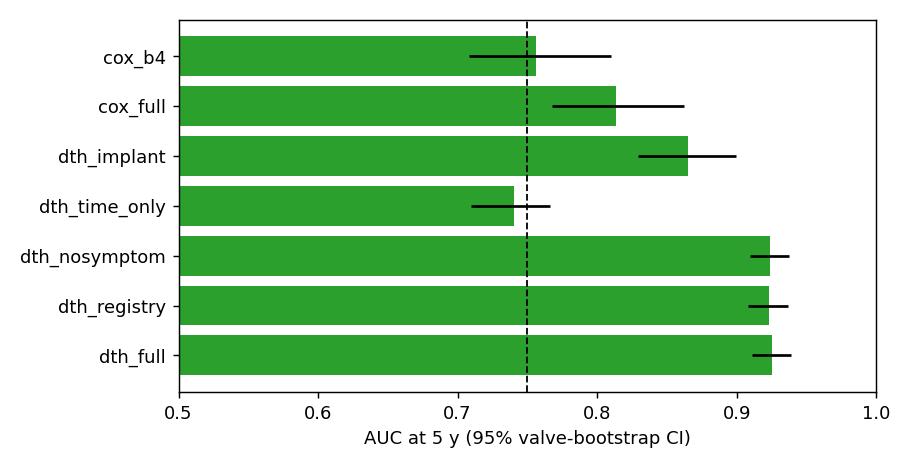
\includegraphics[width=\textwidth]{auc_models_5y}
\caption{Five-year AUC by model with bootstrap intervals; the dashed line is the pre-specified 0.75 threshold. \vt{dth} = discrete-time hazard model.}
\label{fig:auc}
\end{minipage}\hfill
\begin{minipage}[t]{0.38\textwidth}\centering
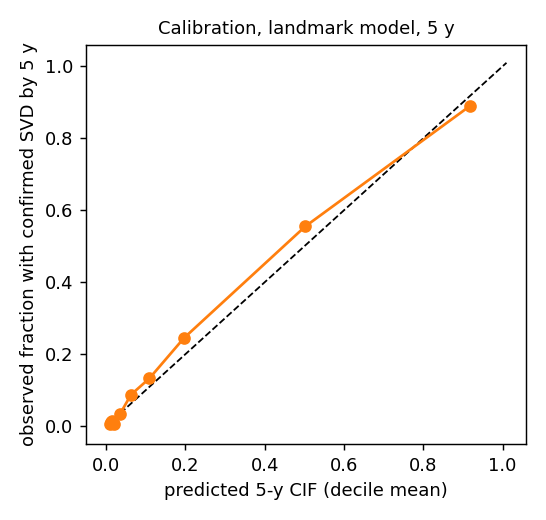
\includegraphics[width=0.9\textwidth]{calibration_5y}
\caption{Decile calibration of the dynamic model at five years.}
\label{fig:calib5}
\end{minipage}
\end{figure}

\textbf{Explainability.} SHAP ranked approach, valve model, prediction horizon, change in gradient from reference, time since implant, age, peak velocity and current haemodynamic stage highest (\cref{fig:shap}). Each inference returns the 5/8/10-year incidence, a tier (low $<5\%$, moderate 5--15\%, high $\geq 15\%$), the top-3 drivers with direction, the recommended interval and flags (unconfirmed abnormal echo, reference from table, valve model with little history). Example from the test set: ``Echo 9.9 y after TAVR: 5-y incidence of confirmed moderate SVD 5.1\% (moderate); drivers: TAVR ($\downarrow$), gradient +4.9 mmHg from reference ($\uparrow$), 9.9 y since implant ($\uparrow$).''

\begin{figure}[t]
\centering
\begin{minipage}[t]{0.44\textwidth}\centering
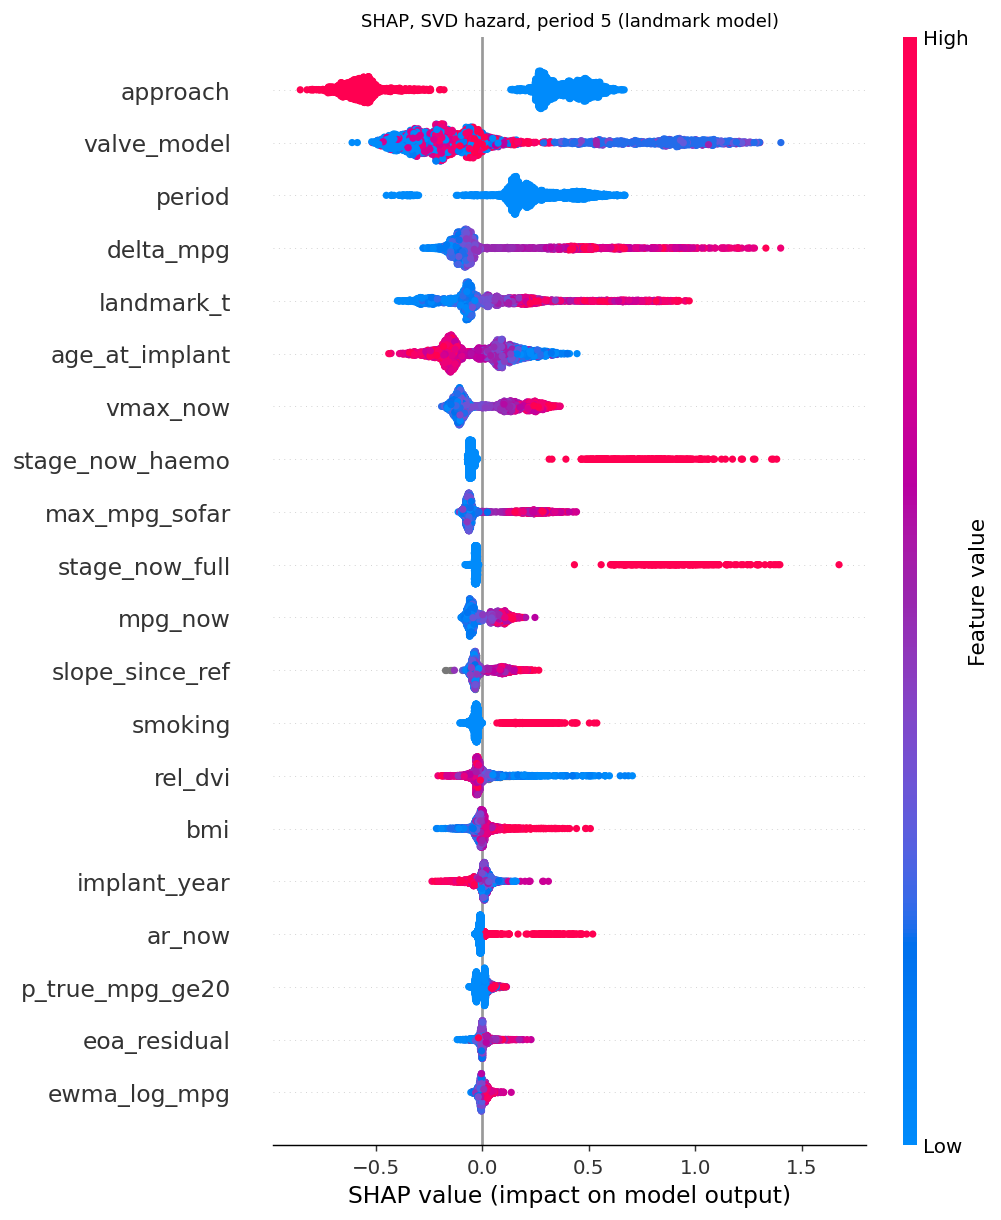
\includegraphics[width=0.85\textwidth]{shap_summary}
\caption{SHAP summary of the dynamic model on the test set.}
\label{fig:shap}
\end{minipage}\hfill
\begin{minipage}[t]{0.52\textwidth}\centering
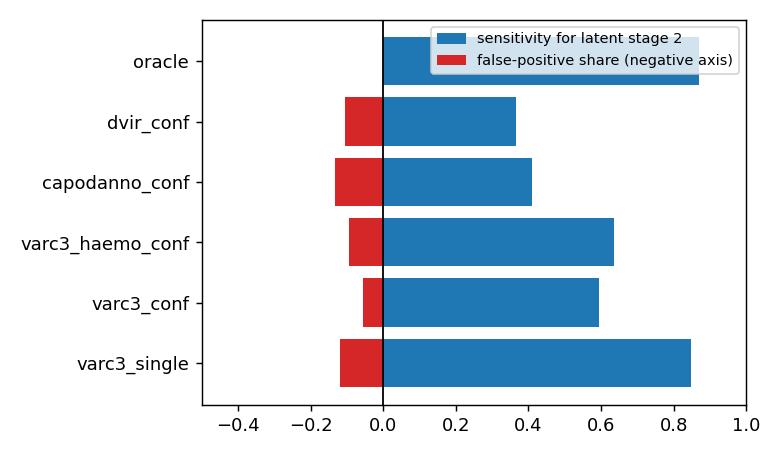
\includegraphics[width=\textwidth]{oracle_definition_audit}
\caption{Each label definition against the noise-free truth: sensitivity for true stage-2 deterioration during follow-up (blue) and share of labels that are false positives (red).}
\label{fig:audit}
\end{minipage}
\end{figure}

\subsection{What the label costs}
Because the simulator keeps the truth, each definition can be audited (\cref{tab:audit}, \cref{fig:audit}). The confirmed VARC-3 label is precise (5.7\% false positives) but detects only 60\% of true moderate deteriorations during follow-up, with a median lag of 1.46 years after the true crossing; the single-echo label is more sensitive but 12\% of its labels are noise; Capodanno and Dvir confirmed labels miss most events. Predicting the noise-free crossing with the same features is \emph{harder} (AUC 0.88) than predicting the observed label (0.925), because the observed label shares measurement noise with the latest echo; AUCs on real echo labels therefore overstate how well true deterioration is anticipated. Trained on the confirmed label, the model transfers across definitions (AUC 0.90--0.94 for the single, haemodynamic, Capodanno and Dvir confirmed labels).

\begin{table}[t]
\centering\small
\caption{Definition audit on the full synthetic cohort against the true stage-2 crossing.}
\label{tab:audit}
\footnotesize
\begin{tabular}{@{}lcccc@{}}
\toprule
Label & Labelled valves & Sensitivity & False-positive share & Median lag (y) \\
\midrule
VARC-3 single echo & 2,504 & 0.85 & 0.12 & 0.55 \\
\textbf{VARC-3 confirmed (primary)} & 1,641 & 0.60 & 0.06 & 1.46 \\
VARC-3 haemodynamic, confirmed & 1,831 & 0.64 & 0.10 & 1.34 \\
Capodanno 2017, confirmed & 1,226 & 0.41 & 0.13 & 1.12 \\
Dvir 2018, confirmed & 1,064 & 0.37 & 0.11 & 1.12 \\
Oracle (noise-free rule at the same visits) & 2,263 & 0.87 & 0.00 & 0.51 \\
\bottomrule
\end{tabular}
\end{table}

\subsection{Subgroups, robustness and sample size}
AUC was 0.908 for SAVR and 0.923 for TAVR; 0.932 in women and 0.919 in men with calibration slopes 0.99 and 0.94; 0.933 with a 30-day reference echo and 0.911 with a table reference. Two valve classes are weaker and are flagged in the output: Trifecta-class (AUC 0.84) and porcine/Mitroflow-class (0.78, calibration slope 0.53), both with early, often regurgitant failure. Under mechanism shifts not seen in training (echo noise $\times 0.5$ and $\times 1.5$, missingness $\times 2$, faster progression) AUC stayed between 0.927 and 0.969. Subsampling the cohort gave 5-year AUC confidence-interval widths of 0.095, 0.050, 0.034 and 0.022 with 500, 1,000, 2,000 and 5,000 valves, which fixes the protocol's target of 5,000 development valves.

\subsection{Surveillance}
\Cref{tab:policy} and \cref{fig:policy} compare the schedules. Two findings stand out. First, the confirmation echo alone is worth a lot: it cuts the mean delay from true onset to confirmed detection from 1.52 to 1.13 years and raises the share of deteriorations detected from 64\% to 73\%, for 4\% more echoes. Second, the risk-adapted schedule at $\tau = 1\%$ used 4.7 echoes per patient-decade instead of 8.4, \textbf{44\% fewer}, with +0.7 months mean and +1.8 months 90th-percentile delay, within the pre-specified 3-month bound; it detected 69\% of deteriorations against 73\%. Thresholds above 3\% save little more and breach the 90th-percentile bound. The oracle (2.1 echoes, 0.94 years delay) shows how far a perfect risk score could go. The model's own value beyond the time-only schedule is modest in mean delay but visible in the tail and in detection rate, which is what the label noise allows.

\begin{table}[t]
\centering\small
\caption{Surveillance policies on identical simulated patients (delay from true stage-2 crossing to confirmed detection).}
\label{tab:policy}
\footnotesize
\begin{tabularx}{\textwidth}{@{}>{\hsize=.9\hsize}Ycccc>{\hsize=1.1\hsize}Y@{}}
\toprule
Policy & Echoes / decade & Detected & Mean delay (y) & P90 delay (y) & vs guideline + confirmation: echoes; mean / P90 delay \\
\midrule
Guideline \cite{praz2025} & 8.06 & 0.64 & 1.52 & 2.87 & $-4\%$; +4.7 / +8.3 mo \\
Guideline + confirmation echo & 8.42 & 0.73 & 1.13 & 2.18 & reference \\
Rule-based de-escalation & 7.62 & 0.70 & 1.17 & 2.25 & $-10\%$; +0.5 / +0.9 mo \\
Time since implant only & 5.20 & 0.68 & 1.28 & 2.45 & $-38\%$; +1.8 / +3.2 mo (P90 fails) \\
\textbf{Risk-adapted, $\tau = 1\%$} & \textbf{4.74} & 0.69 & 1.19 & 2.33 & \textbf{$-44\%$; +0.7 / +1.8 mo} \\
Risk-adapted, $\tau = 2\%$ & 4.38 & 0.67 & 1.25 & 2.37 & $-48\%$; +1.5 / +2.3 mo \\
Risk-adapted, $\tau = 5\%$ & 4.19 & 0.67 & 1.30 & 2.44 & $-50\%$; +2.0 / +3.2 mo (P90 fails) \\
Oracle (sees the truth) & 2.06 & 0.74 & 0.94 & 1.89 & $-75\%$; $-2.3$ / $-3.5$ mo \\
\bottomrule
\end{tabularx}
\end{table}

\begin{figure}[t]
\centering
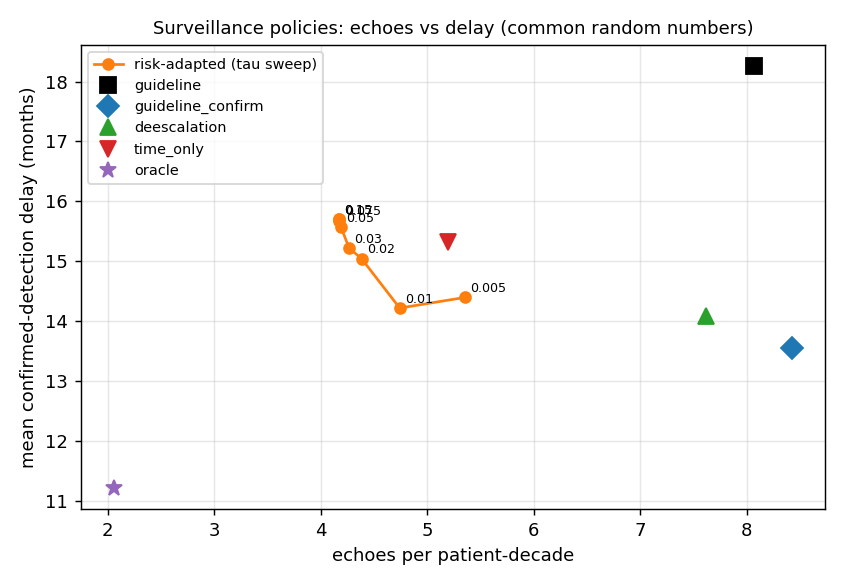
\includegraphics[width=0.66\textwidth]{policy_frontier}
\caption{Echoes used against mean confirmed-detection delay for every policy; the orange curve is the risk-adapted schedule across thresholds $\tau$.}
\label{fig:policy}
\end{figure}

\subsection{Secondary endpoints}
From first confirmed moderate SVD, median time to severe SVD or reintervention was 1.32 years (63\% within two years), shortest for Perimount-, Trifecta- and porcine-class valves (1.1--1.2 years) and longest for self-expanding (2.7) and balloon-expandable (10) valves. BVF cumulative incidence was 4.7/9.8/14.8\% and reintervention 4.1/8.8/13.2\% at 5/8/10 years; about 38\% of reinterventions were urgent under guideline surveillance. Median annualised gradient progression was 0.56 mmHg/year after SAVR and 0.35 after TAVR.

\section{A check on real data}\label{sec:real}

The hackathon's de-identified notes (117 patients) were profiled for what a notes-based pipeline can recover: valve model named in 92\%, size in 97\%, BMI in 47\%, a prosthetic-valve echo with a mean gradient in 36\%, gradients in two different years in 2\%, and a numeric age in none (redacted). We hand-adjudicated 26 patients with a known valve, implant year and documented valve status, 11 of them with documented structural dysfunction, recorded a source quote for each, and ran the trained models on them (\cref{tab:real}).

\begin{table}[t]
\centering\small
\caption{Face-validity check on the provided notes. Not a validation: no serial echoes, year-level dates, ages redacted, failure-enriched sample.}
\label{tab:real}
\footnotesize
\begin{tabularx}{\textwidth}{@{}Yc>{\raggedright\arraybackslash}p{5.6cm}@{}}
\toprule
Check & $n$ (events) & Result \\
\midrule
VARC-3 rule with model~$\times$~size reference vs documented dysfunction & 25 (7) & sensitivity 86\%, specificity 89\% \\
Dynamic model at the follow-up echo, 5-y risk vs documented dysfunction & 20 (5) & AUC 0.97 (0.88--1.00); partly circular \\
\quad surgical valves $\geq 5$ y after implant & 9 (5) & AUC 0.90; single-echo rule alone 0.78 \\
Implant-time boosted model, 10-y risk vs time to documented dysfunction & 26 (11) & C 0.59 (0.36--0.82); uninformative \\
Published risk-factor Cox & 26 (11) & C 0.51 (0.19--0.86) \\
\bottomrule
\end{tabularx}
\end{table}

The label rule behaved as the simulation predicted: both false positives were stable gradients of 21 mmHg that the model~$\times$~size table misreads as a rise (one patient's own earlier echo as reference removes the label), and the one miss was moderate stenosis hidden by low flow. The dynamic model ranked the real failing valves first, but the clinicians diagnosed most of those failures from the very echo the model scored, so this shows recognition, not anticipation. The implant-time result is uninformative: the strongest predictor, age, is redacted everywhere, dates are year-level and there are 11 events. Real validation needs structured serial echoes with exact dates and ages, which is what the protocol requests.

\section{Limitations, ethics and next steps}

\textbf{Limitations.} All performance figures come from a literature-calibrated simulator; they show that the design works and where it breaks, not the expected real-world AUC, which will be lower. The simulator assumes symptoms only with true deterioration, death independent of SVD, and no site or vendor effects; severe SVD progresses slightly too fast; new valve models borrow their class hazard until local events accrue. Even the confirmed label detects only 60\% of true deteriorations with a 1.5-year lag, and the model inherits this ceiling. The engineered trajectory features added little over registry fields in the prototype, and the model's surveillance gain over a time-only rule was modest in mean delay; both may change with real echo noise.

\textbf{Ethics and privacy.} Retrospective development under IRB waiver; analysis on a HIPAA limited data set because time-to-event needs exact intervals; hashed linkage tokens; models trained inside the health system or federated; no patient-level data in artefacts; the public prototype uses synthetic data only. Fairness is reported within sex, age band, race and ethnicity, approach, valve model and size with pre-specified floors; women and small-annulus patients are analysed as an effect-modifier group through PPM. The system schedules surveillance only, never recommends reintervention, and any single abnormal echo triggers a confirmation echo regardless of risk.

\textbf{Next steps.} Run the same code on one institution's echo database linked to STS/TVT (the schema is already registry-shaped), then external validation at a second system; a silent-mode prospective phase; and, if the decision criterion holds, a pragmatic trial of risk-adapted surveillance. Code, data dictionary, calibration and validation reports, and every number in this document are in the repository.

\printbibliography
\end{document}
